\documentclass{article}
\usepackage{graphicx}
\usepackage{fancyhdr}
\usepackage{lipsum}
\usepackage[margin=1in]{geometry} % Set margins to 1 inch
\usepackage{float} % for the [H] specifier
\usepackage{caption}




% Header configuration
\pagestyle{fancy}
\fancyhf{}
\fancyhead[L]{
\includegraphics[height=20pt]{image/usl_logo.png}}
\fancyhead[R]{Dashboard User Manual V1.0}
\fancyfoot[R]{\thepage} % page number in bottom right


\begin{document}

% Cover Page
\begin{titlepage}
    \centering
    \vspace*{2cm}
    
\includegraphics[width=1.0\textwidth]{image/logo_lbfl.png}
    \vspace*{2cm}

    {\Huge Dashboard Application}\\
    
    \vspace*{1cm}
    
    {\LARGE User Manual}
    
    \vspace*{0.5cm}
    
    {\Large version 1.0}
\end{titlepage}

\title{Dashboard Application User Manual}
\author{Unisoft System Limited}
\date{February 05, 2024}


\maketitle



\newpage

% Table of Contents
\tableofcontents

\newpage

% Sections

% Start of Loin
\section{Login}
\textbf{Enter Credential :} \\
To enter the application, the user must input their username and password. The application will determine the appropriate dashboard based on the user's role. A "Submit" button is provided for proceeding.
\begin{figure}[h]
    \centering
    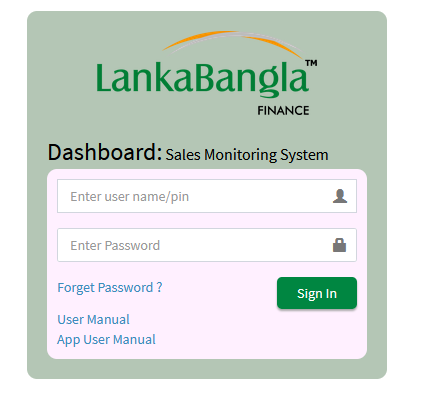
\includegraphics[width=0.75\textwidth]{image/user_login_1.png}
    \caption{Login interface}
\end{figure}


\subsection{Forget Password}
In the event of a password reset, the user is required to input the email address associated with their account. Subsequently, a login token will be dispatched to the provided email address.
\begin{center}
    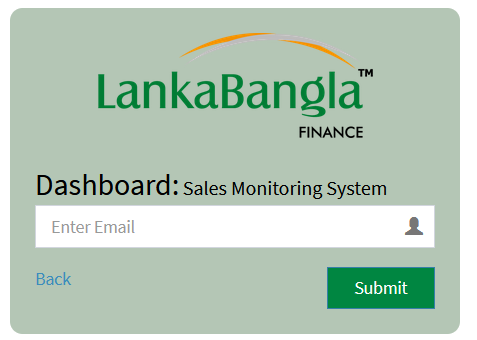
\includegraphics[width=0.75\textwidth]{image/forget_pass_mail_addr.png}
\end{center}


% in case user not found.

\textbf{User not found}\\
In case user not found by email address, in such cases, have to contact with the administrator. 
\begin{center}
    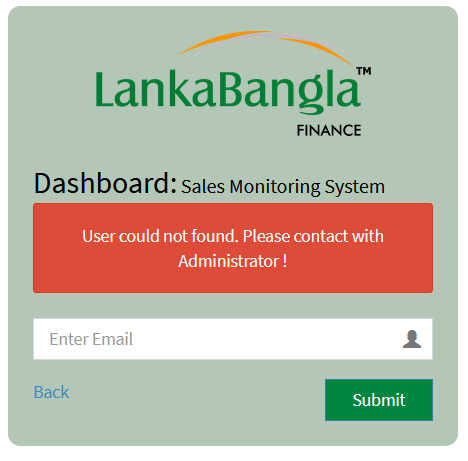
\includegraphics[width=0.75\textwidth]{image/usernot_found_forget_pass.png}
\end{center}

\textbf{Entering the token}\\
When initiating a password reset, a token will be dispatched to the user's email address. Upon receipt of this token, the user is required to enter it into the designated field labeled "Entering the token". Once the token is successfully entered, the system will prompt the user to proceed with the password reset process by displaying the password reset window.
\begin{center}
    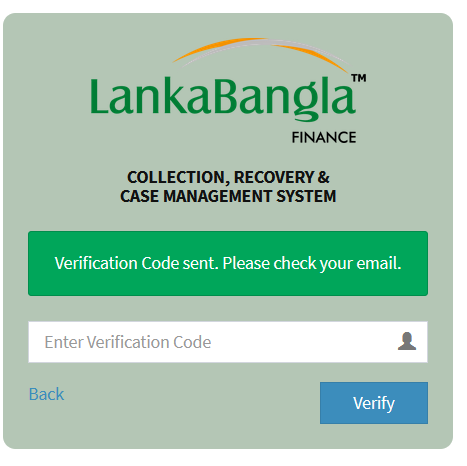
\includegraphics[width=0.75\textwidth]{image/verification_code_send.png}
\end{center}




\subsection{User Manual}
User pdf version of user manual will be downloaded. 

\subsection{App User Manual}
User manual of the mobile app.


% End of Login


\section{Super Admin}
\begin{center}
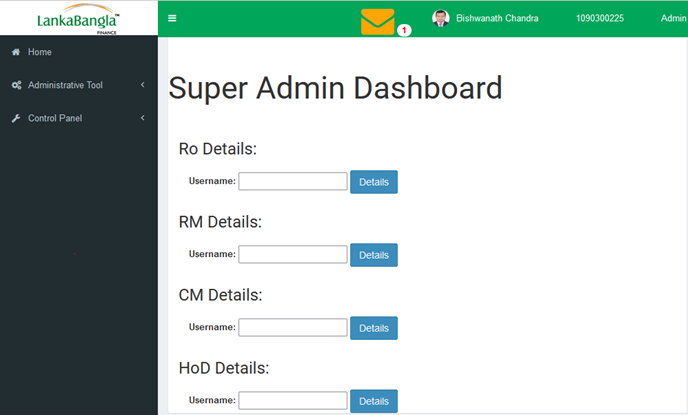
\includegraphics[width=0.75\textwidth]{image/super_admin.png}
\end{center}
In the Super Admin dashboard, the administrator possesses the capability to access the dashboard of any user within the system. To initiate this process, the Super Admin is prompted to input the username corresponding to the desired user type into the provided field. Upon submission, the system redirects the Super Admin to a new tab containing the dashboard associated with the specified user ID.\\

\textbf{If User not found}
\begin{center}
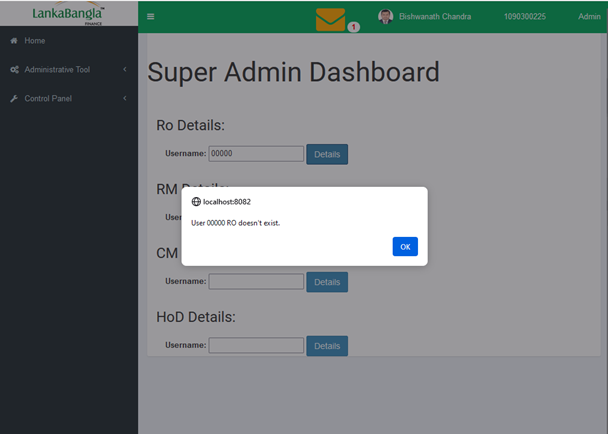
\includegraphics[width=0.75\textwidth]{image/super_admin_user_not_found.png}
\end{center}





% Start of Hod dashboard
\section{HoD Dashboard}

\textbf{HoD view Part 1}\\
\begin{center}
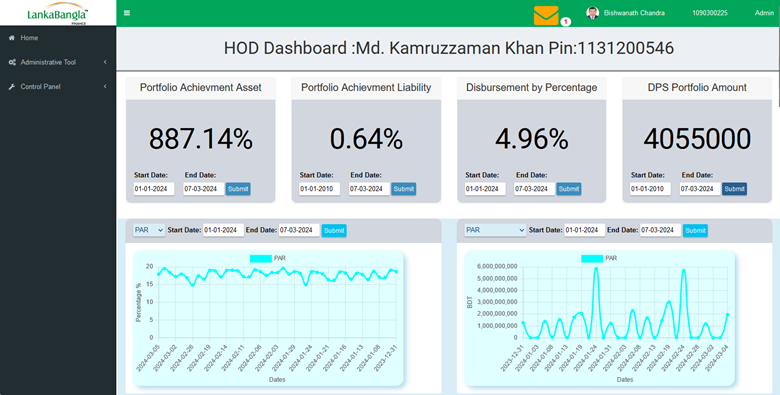
\includegraphics[width=1.0\textwidth]{image/hod_1.png}
\end{center}
\vspace{\baselineskip}
\vspace{\baselineskip}

\textbf{HoD view Part 2}\\
\begin{center}
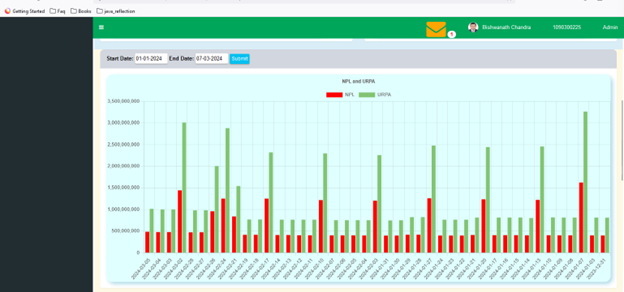
\includegraphics[width=1.0\textwidth]{image/hod_2.png}
\end{center}

\textbf{HoD view Part 3}\\
\begin{center}
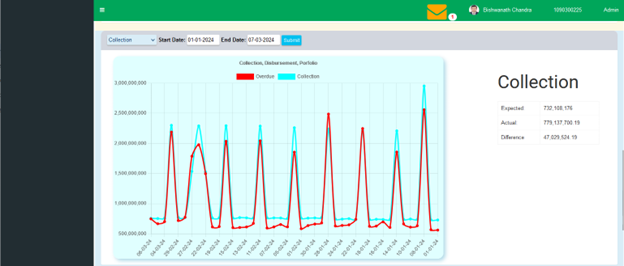
\includegraphics[width=1.00\textwidth]{image/hod_3.png}
\end{center}

\textbf{Team View of the Hod}\\
It is the list of CM under a HOD.
\begin{center}
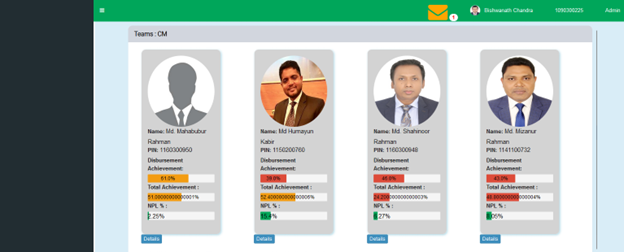
\includegraphics[width=1.0\textwidth]{image/hod_4.png}
\end{center}

% end of hod dashboard



% Start of CM dashboard
\section{CM Dashboard}

\textbf{Team view of CM}
\begin{center}
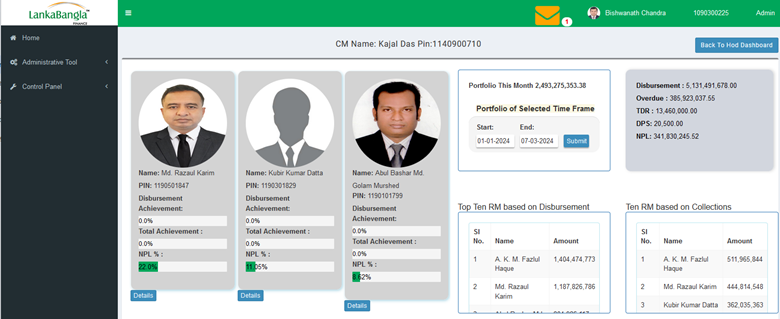
\includegraphics[width=1.0\textwidth]{image/cm_dashboard_image.png}
\end{center}

\textbf{Historical Data of the RM's}
\begin{center}
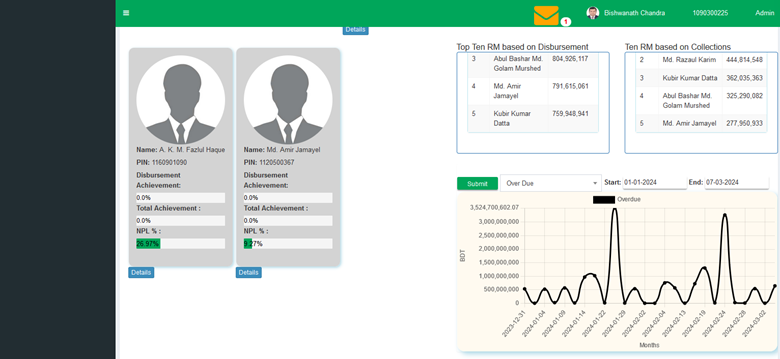
\includegraphics[width=1.0\textwidth]{image/cm_2.png}
\end{center}
% end of CM dashboard


% Start of RM dashboard
\section{RM Dashboard}
\textbf{RM Under the RM}
\begin{center}
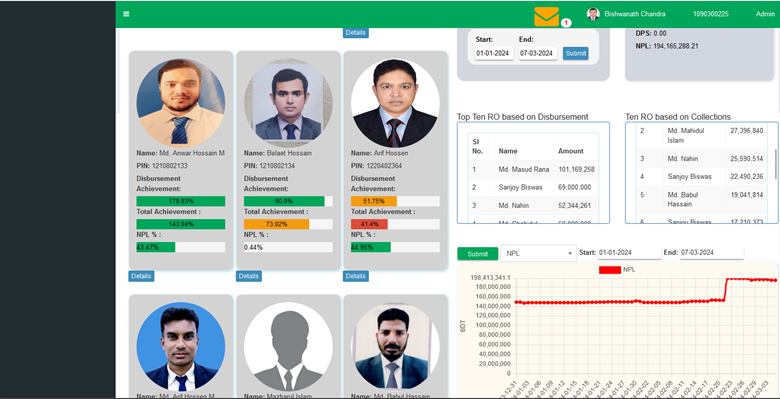
\includegraphics[width=0.75\textwidth]{image/rm_1_team_view.png}
\end{center}
% end of RM dashboard



% Start of RO dashboard
\section{RO Dashboard}
\textbf{RO Dashboard Part 1}
\begin{center}
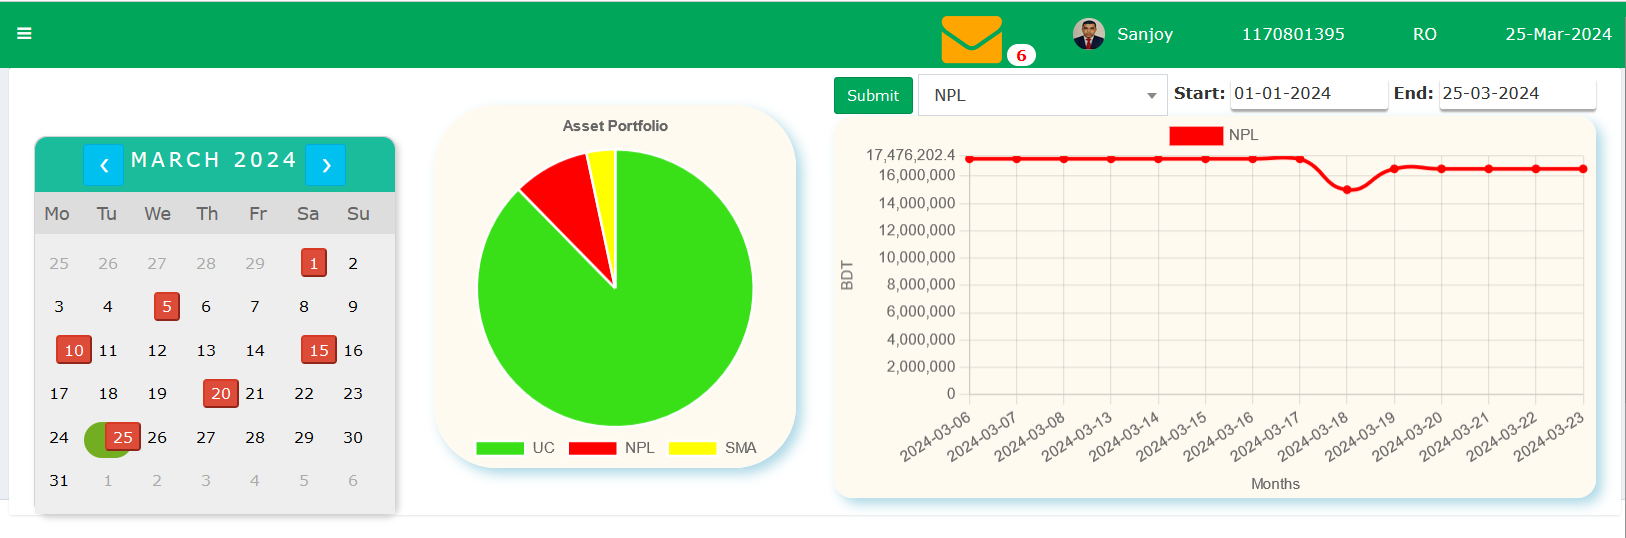
\includegraphics[width=1.0\textwidth]{image/ro_1.png}
\textbf {RO Dashboard : Calender, Asset Portfolio, Graph}
\end{center}


\subsection{Calender}

\begin{center}
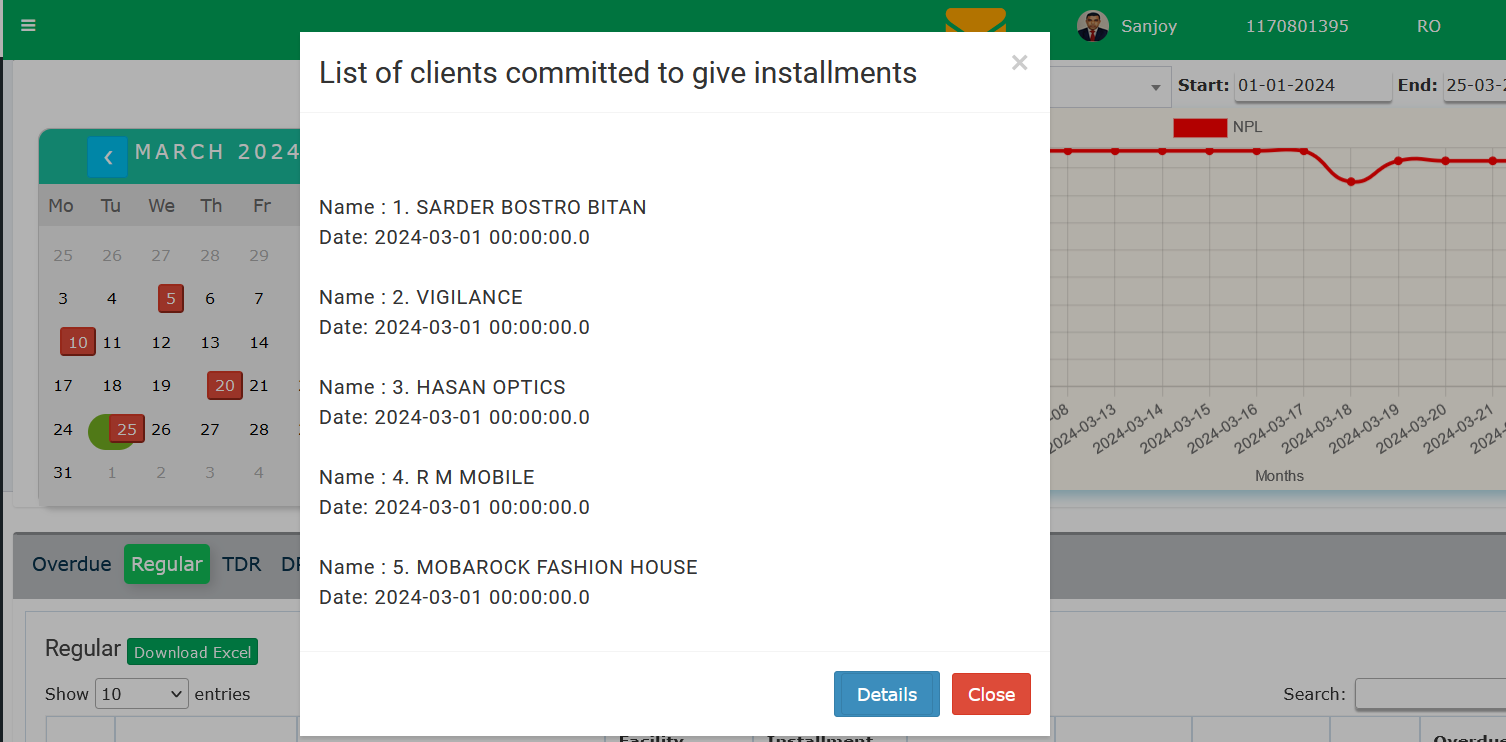
\includegraphics[width=.75\textwidth]{image/ro_3_commited_clients_popup.png}\\
\textbf {Details of the committed clients}
\end{center}

\textbf{ Description : }
The Calendar feature within the software serves as a tool to manage commitments from clients regarding monetary contributions. Dates marked in red signify days where commitments have been made by clients to provide installment payment. Users can interact with these marked dates to view the list of commitments associated with each date. Additionally, users can access detailed information about each commitment through a pop-up window.

\textbf{Accessing the Calendar:} Users can access the Calendar feature from the main menu of the software application. Upon selecting the Calendar option, the calendar interface will be displayed, allowing users to view dates and associated commitments.

\textbf{Viewing Marked Dates:} Within the calendar interface, dates with client commitments are visually highlighted in red to distinguish them from other dates. Users can easily identify these dates by their color.

\textbf{Viewing Commitments:} To view commitments associated with a marked date, users can simply click or tap on the desired date. A pop-up window will appear displaying a list of commitments made by clients for that specific date. Each commitment entry will include relevant details such as client name and date.

\begin{center}
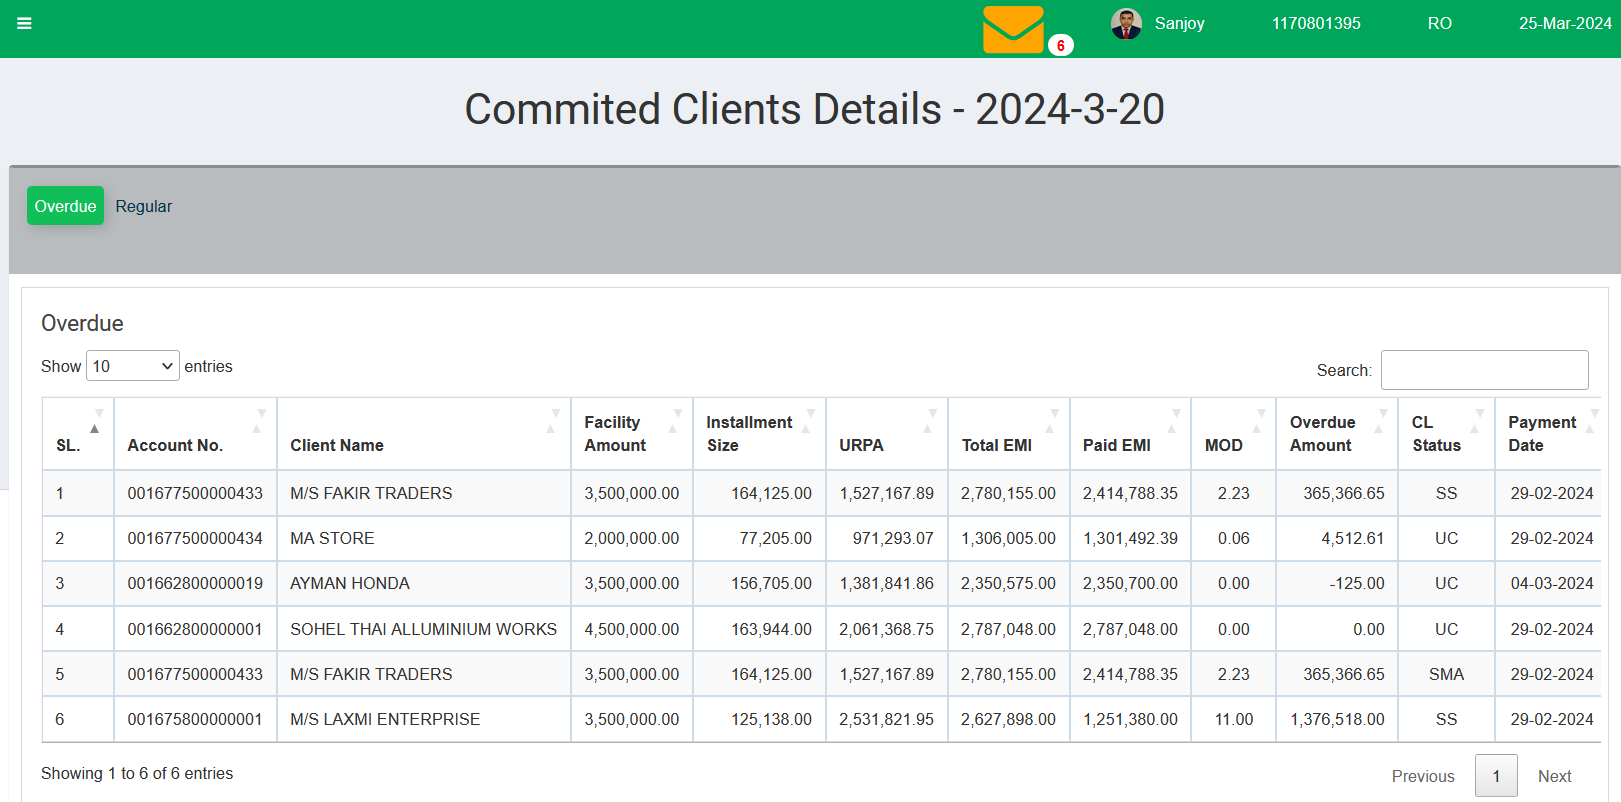
\includegraphics[width=.75\textwidth]{image/ro_4_commited_clients_detailspng.png}\\
\textbf {Details of the committed clients}
\end{center}

\subsection{Asset Portfolio}
\begin{center}
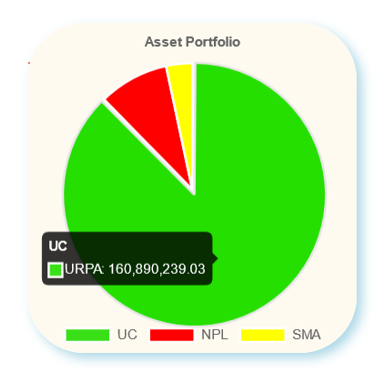
\includegraphics[width=.75\textwidth]{image/ro_5_portfilo_asset.png}\\
\textbf {Asset Portfolio}
\end{center}

\subsection{Graph}
\textbf{Introduction}
The Data Visualization Tool is designed to provide users with a comprehensive view of various segments within a dataset. Through this tool, users can analyze data trends over specific periods, allowing for informed decision-making. The tool offers a graphical representation of the data, making it easier for users to interpret and draw insights.

\textbf{Dropdown Menu:}
The tool provides a dropdown menu with the following options:
\begin{itemize}
    \item Segment
    \item Over Due
    \item Disbursement
    \item Portfolio
    \item Collection
    \item Regular
    \item UC
    \item SMA
    \item NPL
    \item TDR
    \item DPS
\end{itemize}

\textbf{Date Selection:} Users can specify a start date and an end date to define the range for data analysis. By default, the start date is set to the beginning of the current year, providing year-to-date data analysis.
\textbf{Graphical Representation:} The tool generates graphical representations, such as graphs and charts, to visualize the selected data. This visual aid helps users to identify trends, patterns, and anomalies within the dataset.



\textbf{RO Dashboard Part 2}
\begin{center}
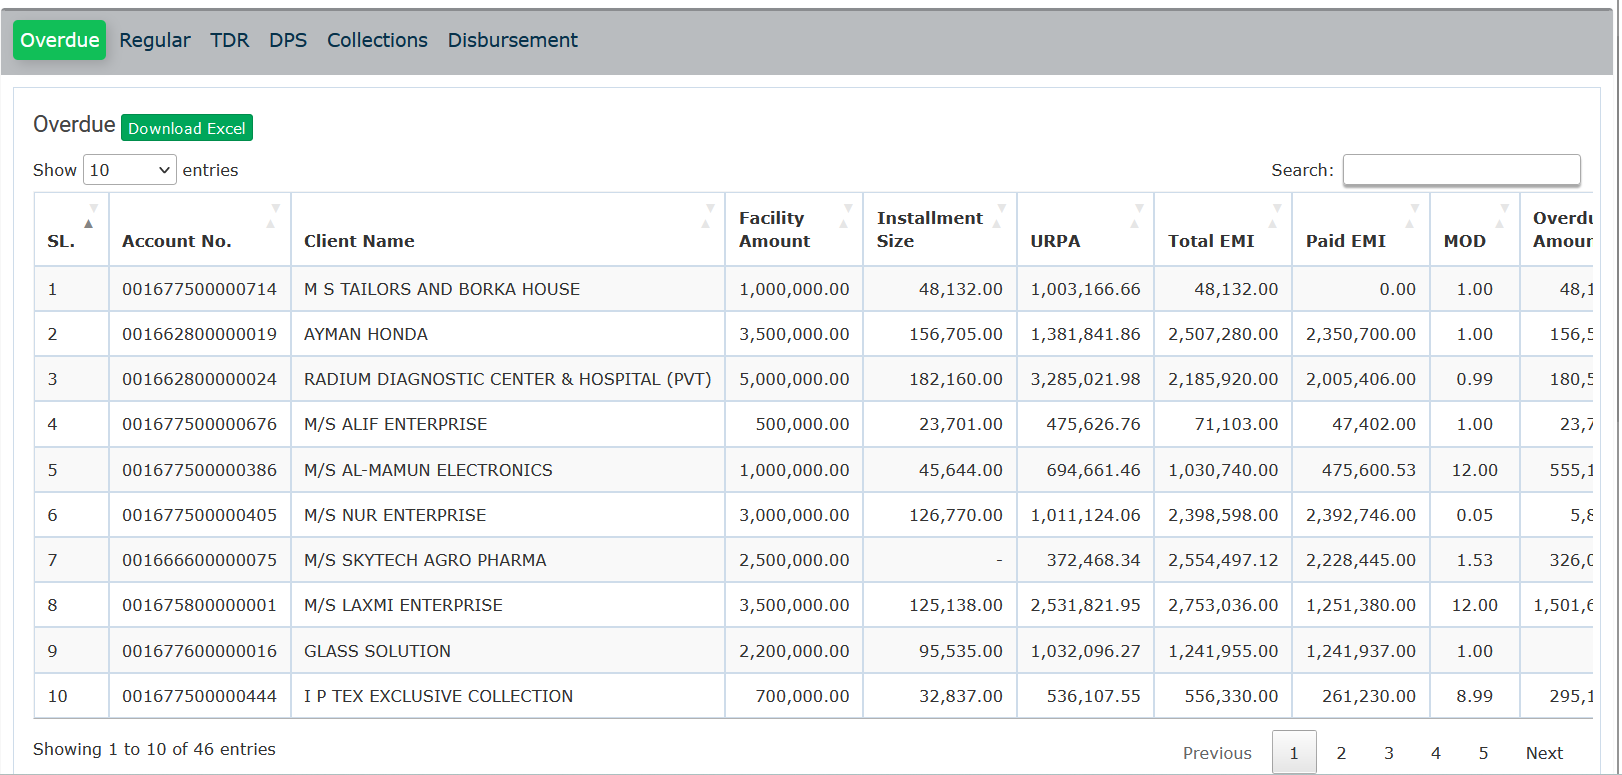
\includegraphics[width=1.0\textwidth]{image/ro_2.png}
\end{center}

\textbf{Download}\\
Clicking on the download button, current tab data will be downloaded in Excel format. 

\begin{center}
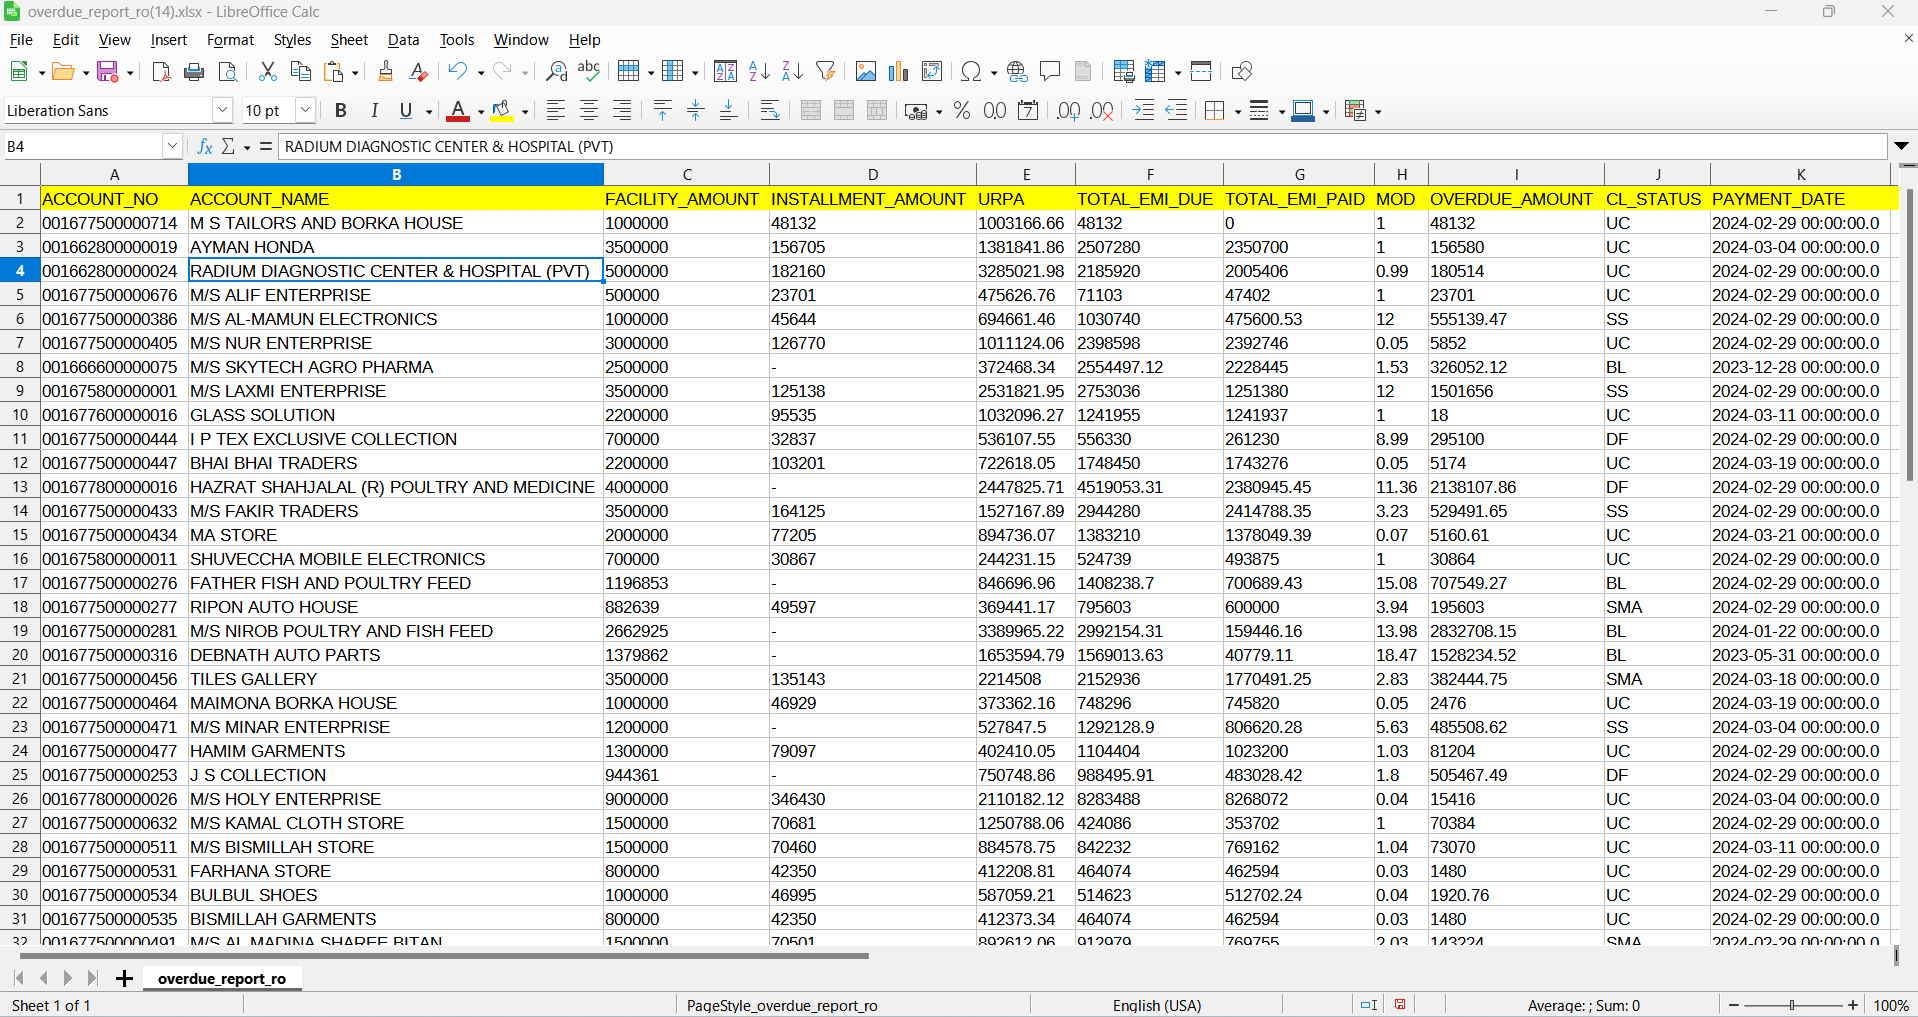
\includegraphics[width=1.0\textwidth]{image/ro_6_sample_excel.png}
\textbf{Sample of the excel}
\end{center}

\section{Change Password}
\begin{center}
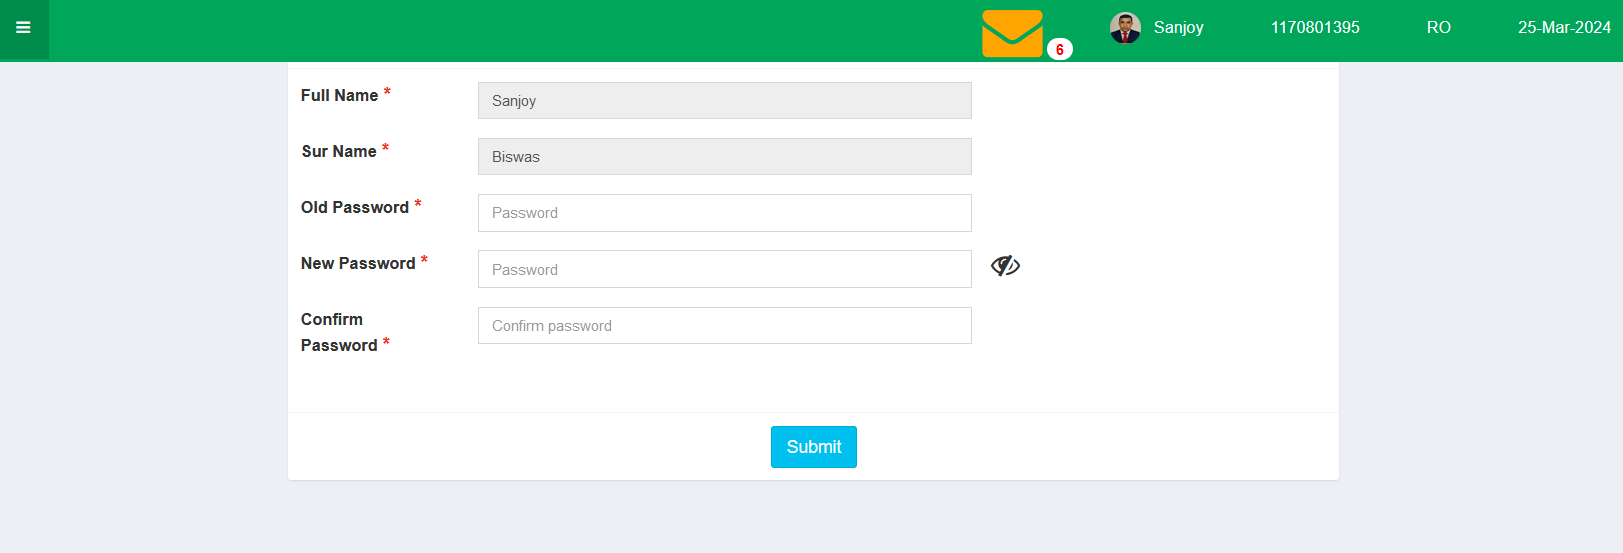
\includegraphics[width=1.0\textwidth]{image/change_password.png}
\textbf{Change Password}
\end{center}

\textbf{Change Password}\\
\textbf{Enter Old Password:}\\
In the designated field, enter your current or old password. This serves as a security measure to verify your identity and ensure that only authorized users can change their passwords.

\textbf{Enter New Password:}\\
In the provided text field, enter your desired new password. Ensure that your new password meets any specified requirements regarding length, complexity, and special characters.

\textbf{Confirm New Password:}\\
To confirm the new password, re-enter it in the designated "Confirm Password" field. This step helps prevent typos and ensures that the new password matches the intended one.

\textbf{Password Matching Verification:}\\
As you type the new password and confirm it, the system automatically checks whether the two entries match. If they do not match, an error message should be displayed, indicating that the passwords do not match.

\textbf{Activate Submit Button:}\\
The "Submit" or "Save Changes" button will only be activated once the new password and confirm password fields match. This prevents users from submitting mismatched passwords accidentally.




\end{document}
